\documentclass[12pt]{article}


\usepackage{amssymb}
\usepackage{amsmath}
\usepackage{fullpage}
\usepackage{epsfig}
\usepackage{epstopdf}
\everymath{\displaystyle}
\usepackage{enumerate}

\newif\ifans

\anstrue

\begin{document}

\begin{center}
\underline{\LARGE{Chapter 3.5: Trigonometric Equations}}
\end{center}

\subsection*{Expected Skills:}

\begin{itemize}

\item Be able to solve trigonometric equations.

\end{itemize}

\subsection*{Practice Problems: }

{\bf For problems 1-7, find all values of $\theta$ which satisfy the following equations.}

\begin{enumerate}

\item $2\sin{x}+\sqrt{3}=0$

\ifans\fbox{$\theta=\frac{4\pi}{3}+2\pi k$ or $\theta=\frac{5\pi}{3}+2\pi k$, where $k$ is any integer.} \fi

\item $2\cos^2\theta-\cos\theta-1=0$

\ifans\fbox{$\theta=\frac{2\pi}{3}+2\pi k$, $\theta=\frac{4\pi}{3}+2\pi k$, or $\theta=2\pi k$, where $k$ is any integer.} \fi

\item $\sin(2\theta)+\cos{\theta}=0$

\ifans\fbox{$\theta=\frac{\pi}{2}+\pi k$, $\theta=\frac{7\pi}{6}+2\pi k$, or $\theta=\frac{11\pi}{6}+2\pi k$, where $k$ is any integer.} \fi

\item $\sin\theta-\cos{(2\theta)}=0$

\ifans\fbox{$\theta=\frac{3\pi}{2}+2\pi k$, $\theta=\frac{\pi}{6}+2\pi k$, or $\theta=\frac{5\pi}{6}+2\pi k$, where $k$ is any integer.} \fi

\item $\sec^2\theta-2=0$

\ifans\fbox{$\theta=\frac{\pi}{4}+\frac{\pi}{2}k$, where $k$ is any integer.} \fi

\item $\left|\tan{\theta}\right|=\sqrt{3}$

\ifans\fbox{$\theta=\frac{\pi}{3}+\pi k$ or $\theta=\frac{2\pi}{3}+\pi k$, where $k$ is any integer.} \fi

\item $\tan{4\theta}=-1$

\ifans\fbox{$\theta=\frac{3\pi}{16}+\frac{\pi}{4}k$, where $k$ is any integer.}\fi

\end{enumerate}

In Math 122, you will study the polar coordinate system.  In the polar coordinate system, we identify the location of a point in the plane as an ordered pair $(r,\theta)$ where $r$ is the distance of the point from the origin and $\theta$ is the angle from the positive $x$-axis.  In this coordinate system, we often describe curves by expressing $r$ as a function of $\theta$, $r=f(\theta)$.

\begin{enumerate}
\setcounter{enumi}{7}


\item The curve $r=2-2\cos\theta$ is called a cardioid, shown in red below.  The curve $r=3$ is the blue circle shown below.
\begin{center}
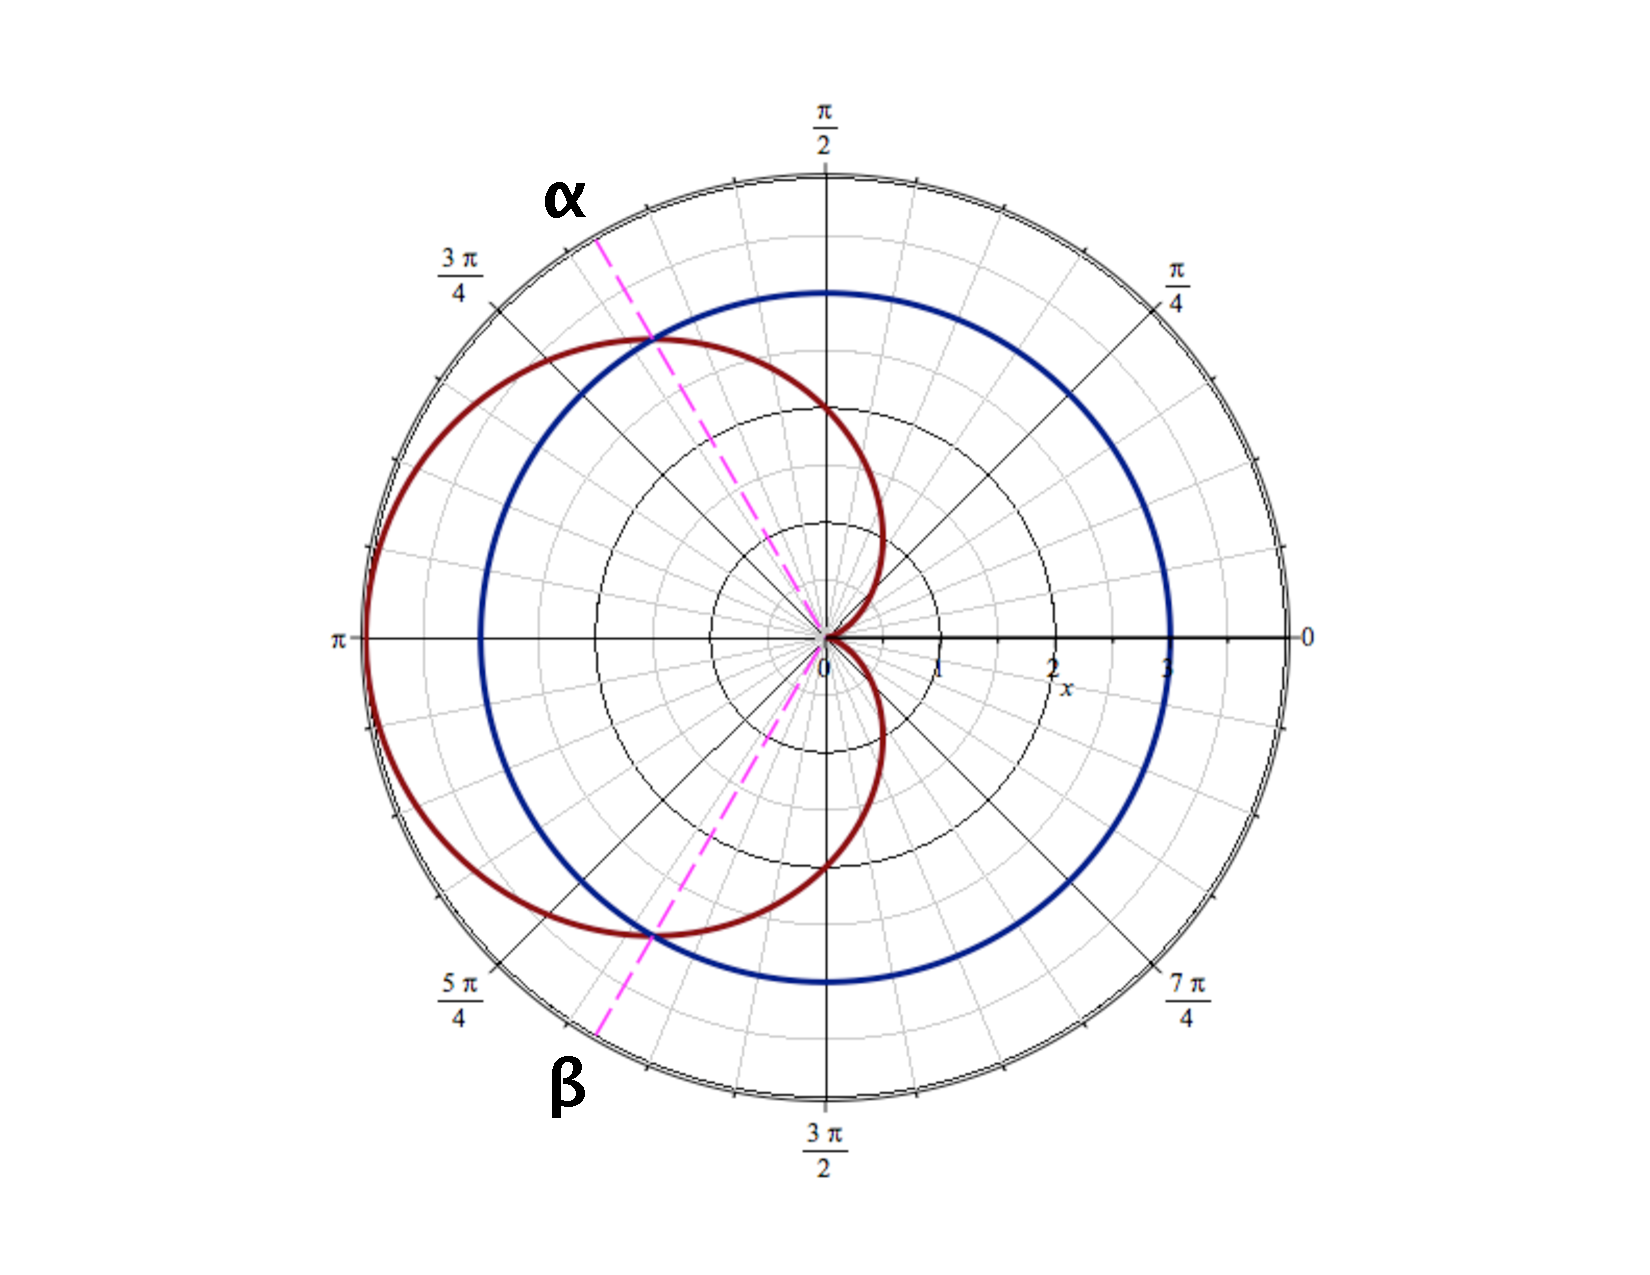
\includegraphics[scale=0.3]{cardioid.pdf}
\end{center}

Find the angles $\alpha$ and $\beta$ at which these curves intersect where $0<\alpha<\beta< 2\pi$

\ifans\fbox{$\alpha=\frac{2\pi}{3}$ and $\beta=\frac{4\pi}{3}$} \fi

\item The curve $r=\sin{(3\theta)}$ describes the rose, shown below.
\begin{center}
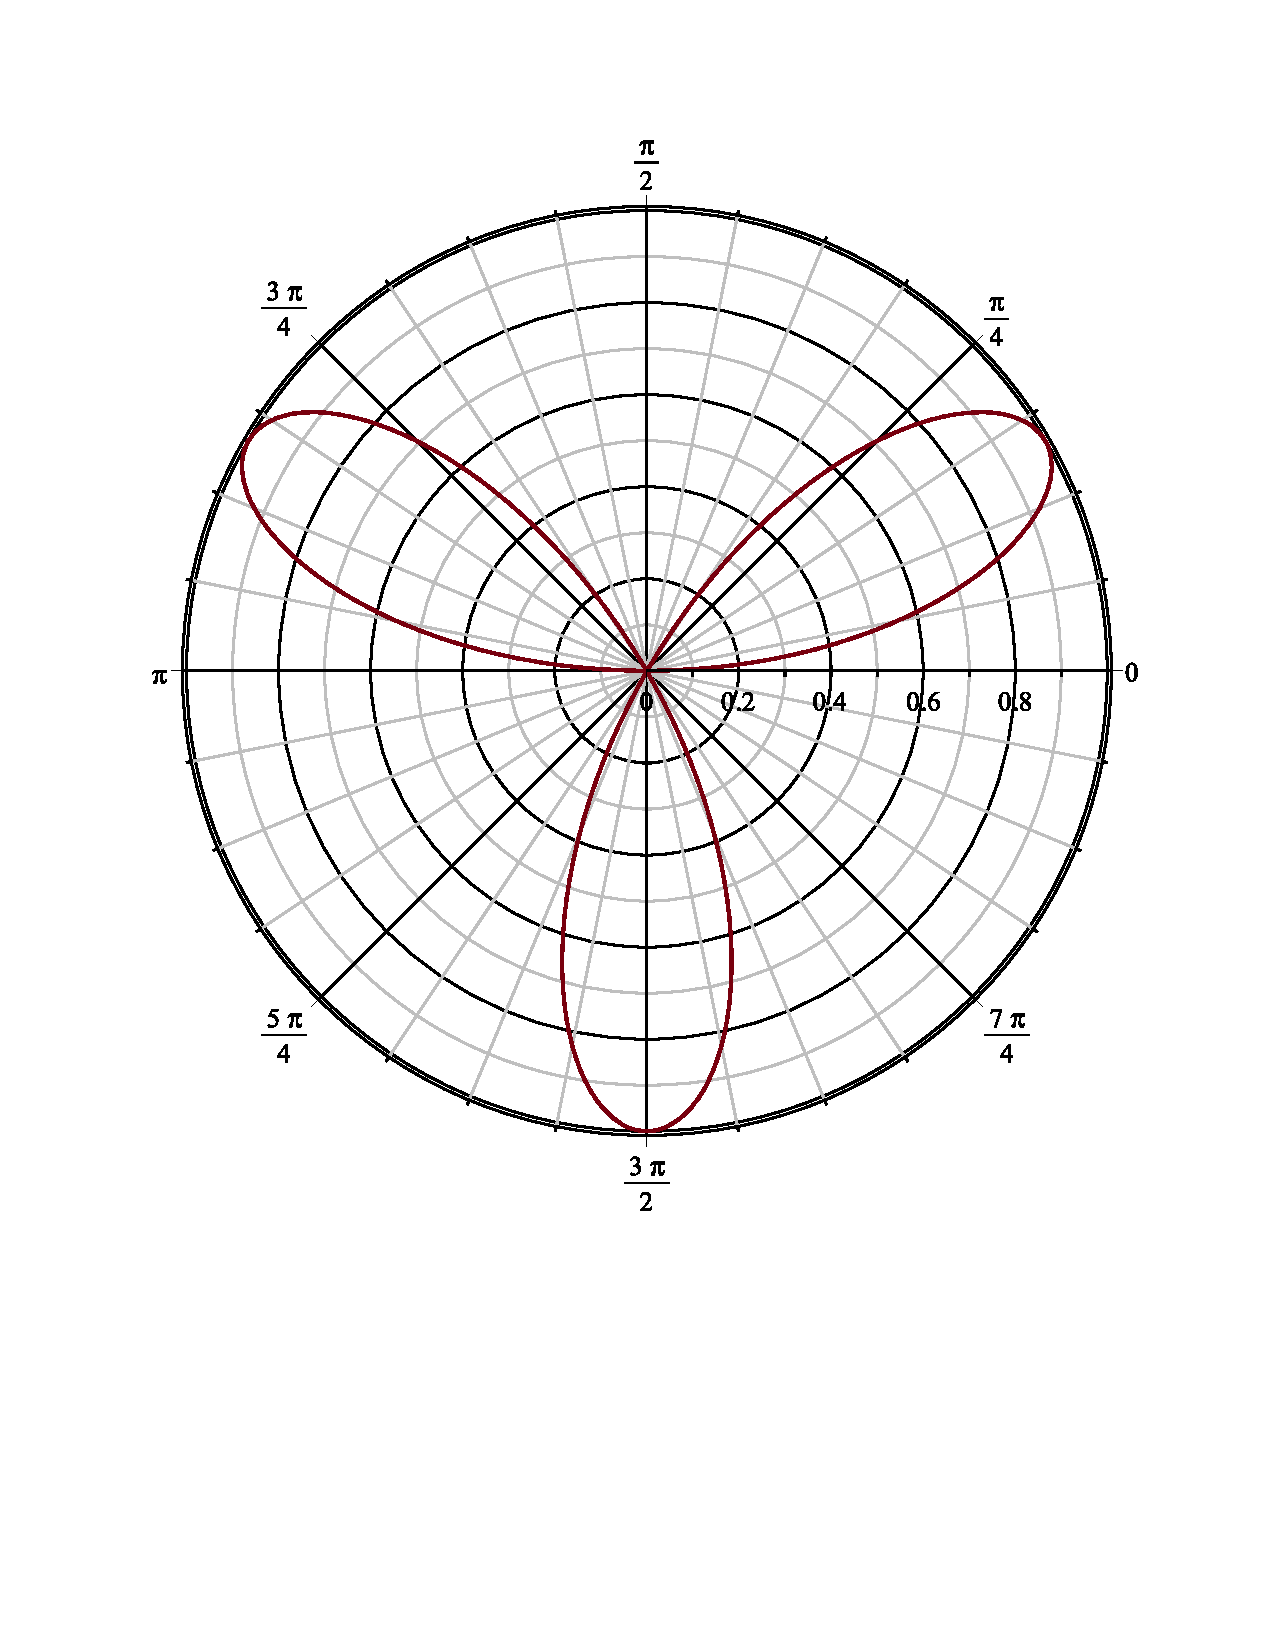
\includegraphics[scale=0.3]{rose.pdf}
\end{center}

\begin{enumerate}

\item Find all values of $\theta$ in the interval $[0,\pi]$ at which the curve passes through the origin.  (Hint: At these points, $r=0$.)

\ifans\fbox{$\theta=0, \frac{\pi}{3}, \frac{2\pi}{3}, \pi$} \fi

\item Find all values of $\theta$ in the interval $[0,\pi]$ which correspond to the ``tips" of the rose petals.  (Hint: At these points, either $r=1$ or $r=-1$.)

\ifans\fbox{$\theta=\frac{\pi}{6}, \frac{\pi}{2}, \frac{5\pi}{6}$} \fi

\end{enumerate}


\end{enumerate}

\end{document}